\documentclass{article}
\usepackage[utf8]{inputenc}
\usepackage{amsmath, amssymb, amsthm, cancel}
\usepackage{enumitem}
\usepackage{caption}
\usepackage{graphicx}
\usepackage[top=1in, bottom=1in, left=1in, right=1in]{geometry}
\usepackage{float}
\usepackage{booktabs}
\usepackage{array}
\usepackage{multirow}

\title{\textbf{CSCI4150U: Data Mining}\\Anomaly Detection}
\author{Syed Naqvi \\ Student ID: 100590852}
\date{\today}

\begin{document}

\maketitle

\begin{abstract}
This report analyzes the effectiveness of Anomaly Detection using Parametric Models, Distance-based models and Density-based Models. When the
dataset is roughly normally distributed, Mahalanobis distance provides an effective way to identify anomalies. In the case of more abstract
distributions, anomalies can be detected using largest distance to k$^{th}$ nearest neighbor, or minimal density.  
\end{abstract}
    
    

\section{Introduction}

\subsection{Methodology}
First we use Mahalanobis distance to identify outliers on the \textit{G-data} dataset as this dataset follows a roughly normal distribution. We then
use a distance based approach to assign points an anomaly score using the maximal distance from their $k^{th}$ nearest neighbors for $k=[1,2,5]$. The
points with the highest anomaly scores have the highest likelihood of being outliers. Finally, we use the inverse of each of the previous distances
and then the inverse of the average of all k nearest distances for each point to assign density scores. The points with the lowest density score
have the highest chance of being anomalies.  

\subsection{Preprocessing}
To initialize our dataset for clustering, we perform feature standardization and remove the existing labels
column giving the following initial plots:
\begin{figure}[H]
    \centering
    \begin{minipage}[b]{0.49\textwidth}
        \centering
        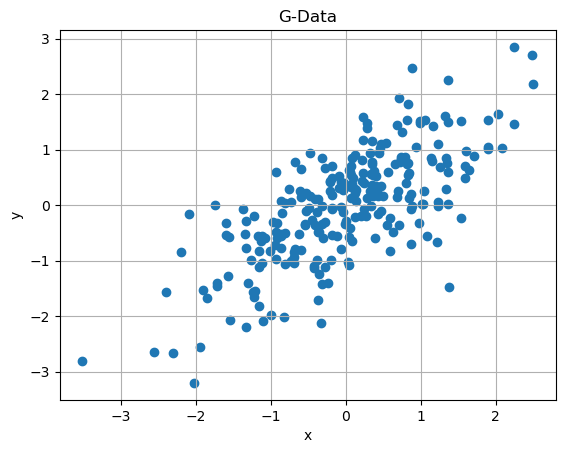
\includegraphics[width=\textwidth]{ea.png}
        \caption{Compound Data}
    \end{minipage}
    \hfill
    \begin{minipage}[b]{0.49\textwidth}
        \centering
        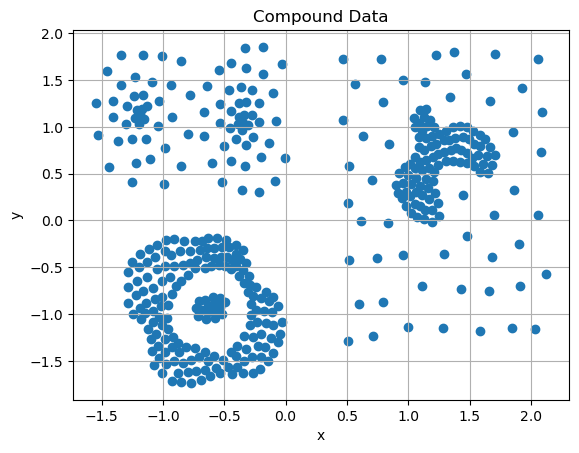
\includegraphics[width=\textwidth]{eb.png}
        \caption{Flame Data}
    \end{minipage}
\end{figure}
\begin{figure}[H]
    \centering
    \begin{minipage}[b]{0.49\textwidth}
        \centering
        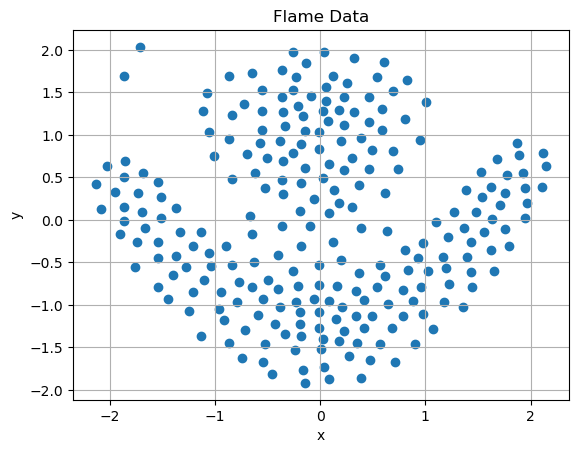
\includegraphics[width=\textwidth]{ec.png}
        \caption{Pathbased Data}
    \end{minipage}
    \hfill
    \begin{minipage}[b]{0.49\textwidth}
        \centering
        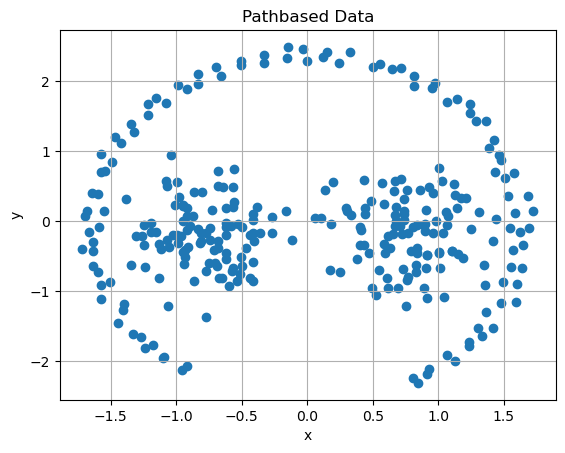
\includegraphics[width=\textwidth]{ed.png}
        \caption{Spiral Data}
    \end{minipage}
\end{figure}

\section{Part I (Using Parametric Models):}
\begin{figure}[H]
    \centering
    \begin{minipage}[b]{0.59\textwidth}
        \centering
        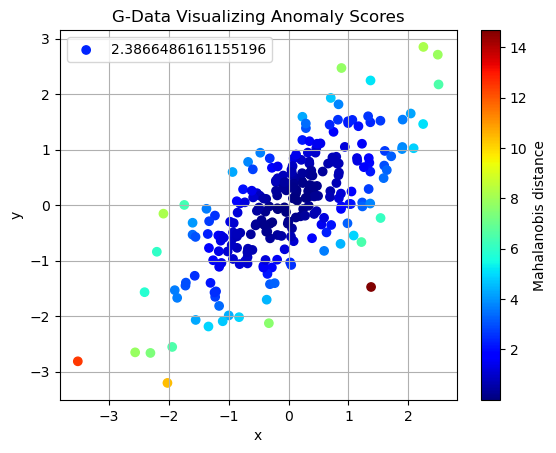
\includegraphics[width=\textwidth]{p1_p.png}
        \caption{G-Data Anomaly Visualization}
    \end{minipage}
    \hfill
    \begin{minipage}[b]{0.4\textwidth}
        \centering
        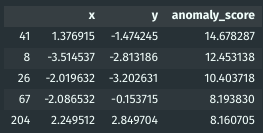
\includegraphics[width=\textwidth]{p1_d.png}
        \caption{G-Data top 5 Anomalies}
    \end{minipage}
\end{figure}

As expected, we see that points along the distribution are penalized less than points
off-distribution. This is evident in some points being a darker red color (higher anomaly score)
despite being closer to the central cluster than other points in a euclidean sense, but actually
being farther off from the main distribution of the dataset. 

\newpage

\section{Part II (Using Distance-Based Models):}
\begin{figure}[H]
    \centering
    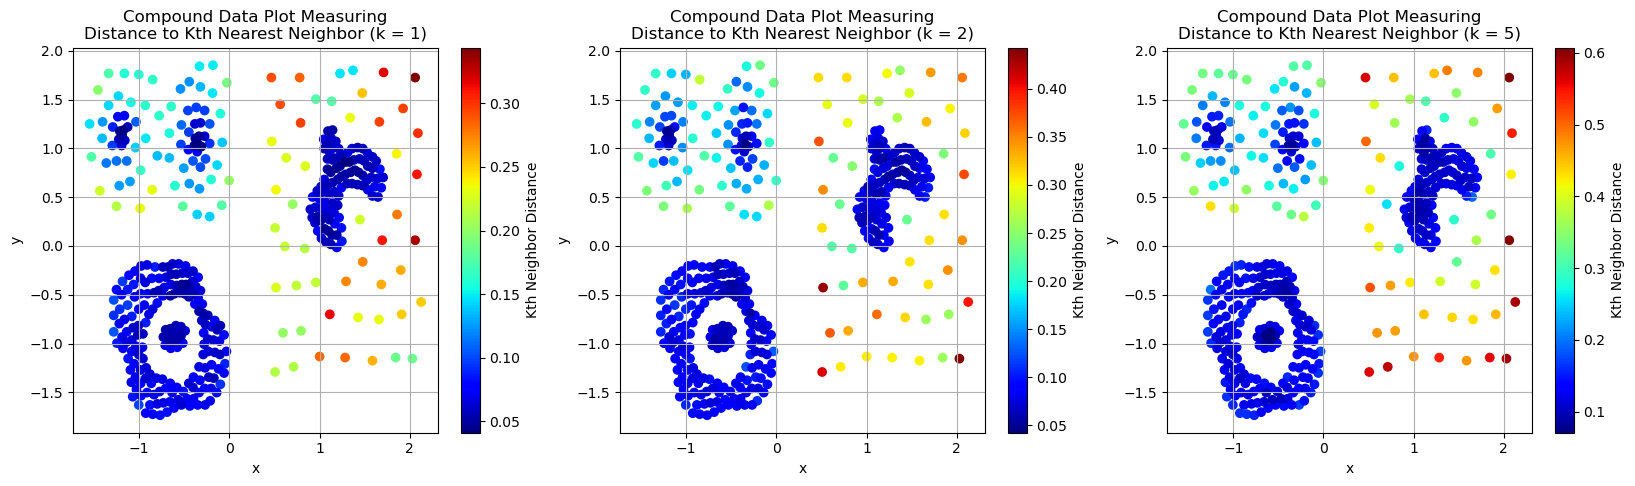
\includegraphics[width=\textwidth]{p2_p1.png}
    \caption{Compound Data Anomaly Visualizations}
\end{figure}
\begin{figure}[H]
    \centering
    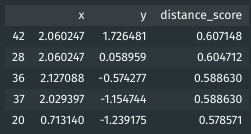
\includegraphics[width=0.4\textwidth]{p2_d1.png}
    \caption{Anomalies with Highest K$^{th}$ Distance (k = 5)}
\end{figure}

Using distance from the 5th nearest neighbor as an anomaly score seems to identify the most intuitive points,
farthest from the main, most compact clusters of the dataset.

\begin{figure}[H]
    \centering
    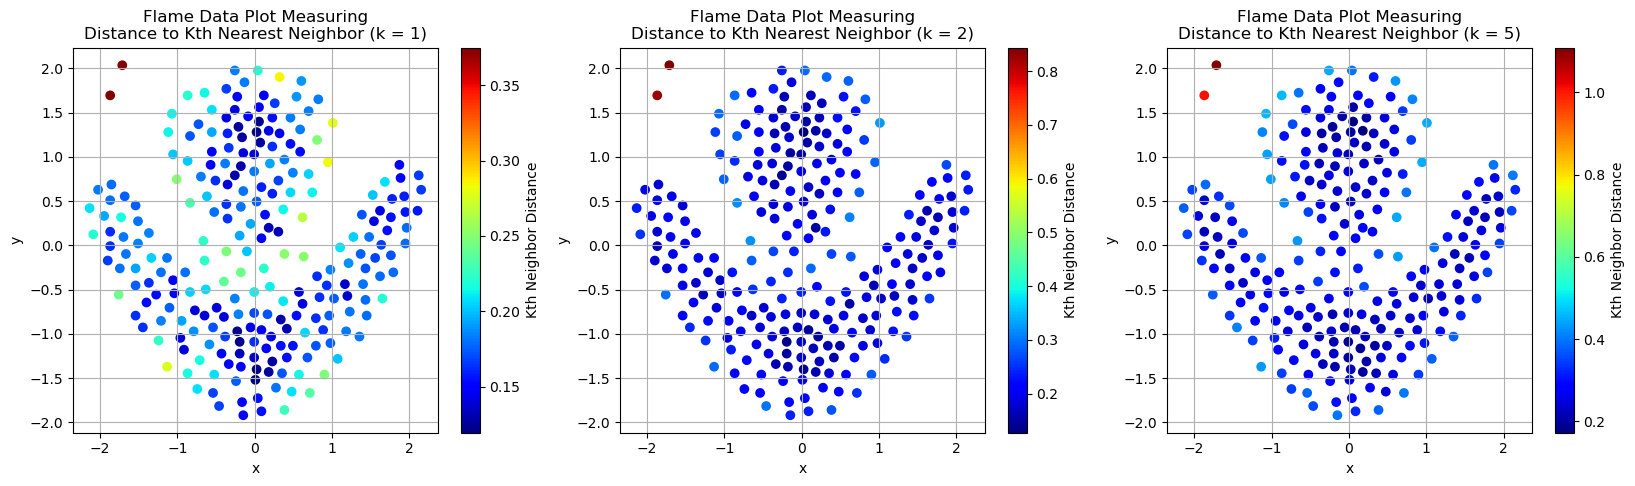
\includegraphics[width=\textwidth]{p2_p2.png}
    \caption{Flame Data Anomaly Visualizations}
\end{figure}
\begin{figure}[H]
    \centering
    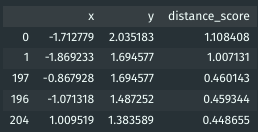
\includegraphics[width=0.4\textwidth]{p2_d2.png}
    \caption{Flame Data Top 5 Anomalies (k = 5)}
\end{figure}

Using distance from the 5th nearest neighbor as an anomaly score seems to identify the most intuitive points,
farthest from the main, most compact clusters of the dataset.

\begin{figure}[H]
    \centering
    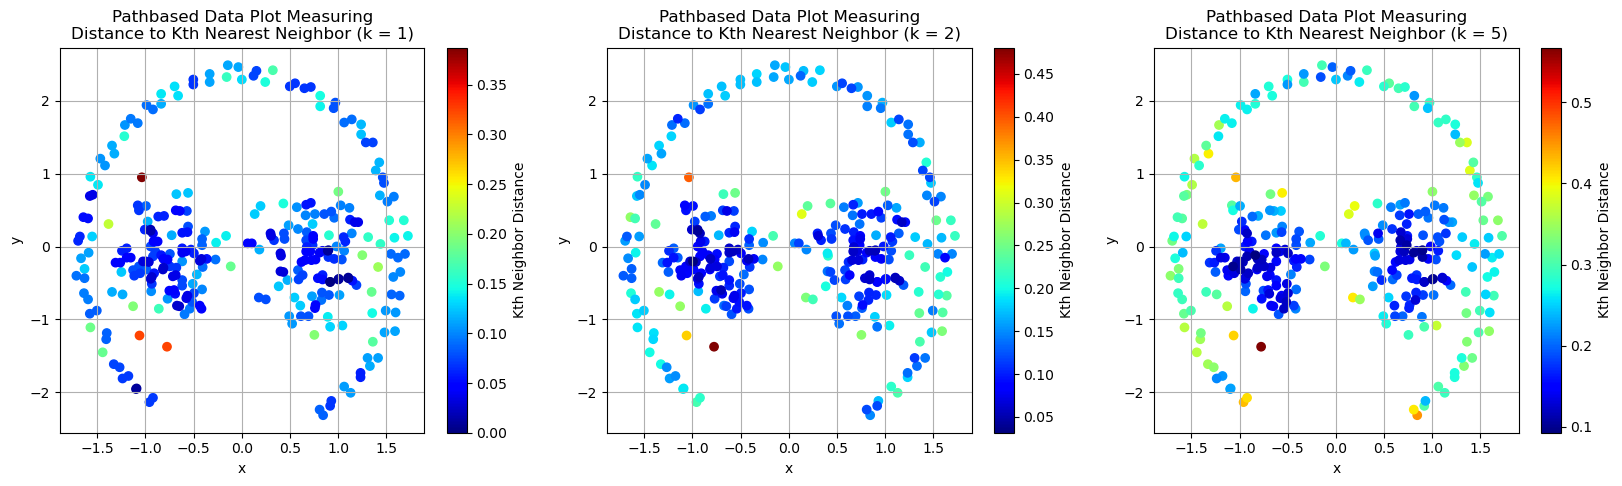
\includegraphics[width=\textwidth]{p2_p3.png}
    \caption{Pathbased Data Anomaly Visualizations}
\end{figure}
\begin{figure}[H]
    \centering
    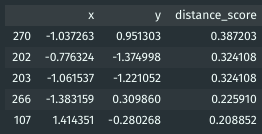
\includegraphics[width=0.4\textwidth]{p2_d3.png}
    \caption{Pathbased Data Top 5 Anomalies (k = 1)}
\end{figure}

In the case of the pathbased dataset, the distance to the first nearest neighbor seems to
do the best job identifying anomalies. This anomaly score was able to remain low for all the
points falling within the two central clusters as well as the bordering ring shape while
identifying points that deviated most from these two distributions.


\section{Part III (Using Density-Based Models):}
\subsection{A. Density as the Inverse of the k$^{th}$ Nearest Neighbor}
\begin{figure}[H]
    \centering
    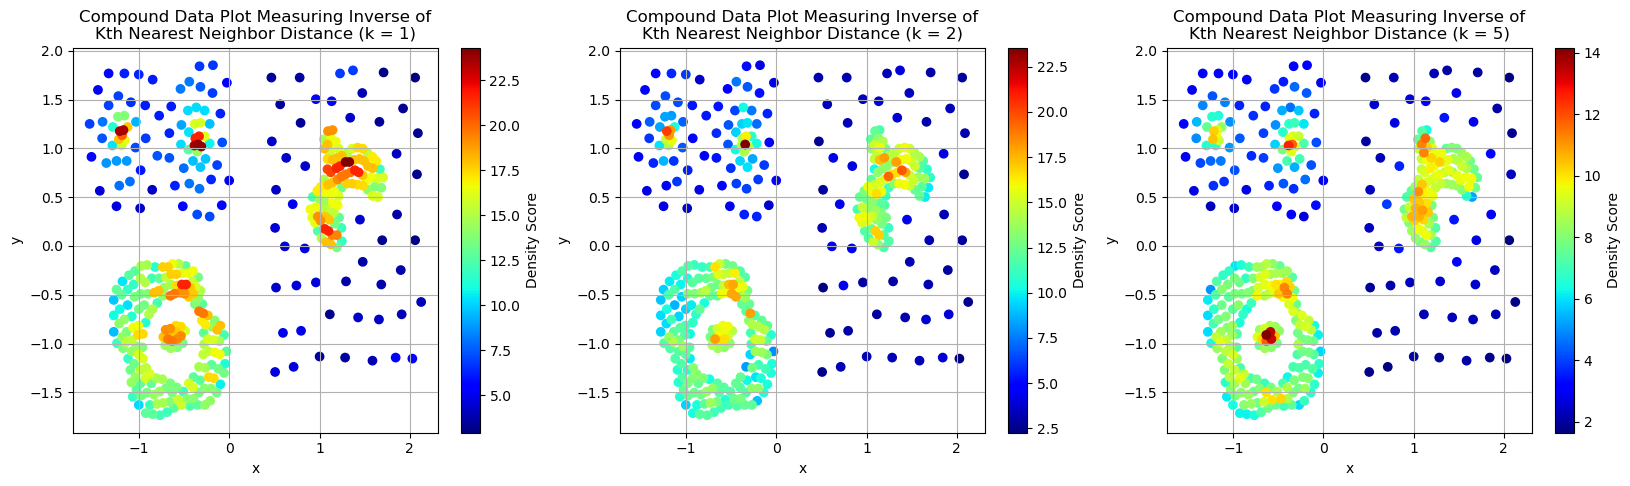
\includegraphics[width=\textwidth]{p3_p1a.png}
    \caption{Compound Data Anomaly Visualizations}
\end{figure}
\begin{figure}[H]
    \centering
    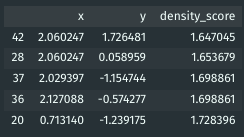
\includegraphics[width=0.4\textwidth]{p3_d1a.png}
    \caption{Compound Data Top 5 Anomalies (k = 5)}
\end{figure}

\begin{figure}[H]
    \centering
    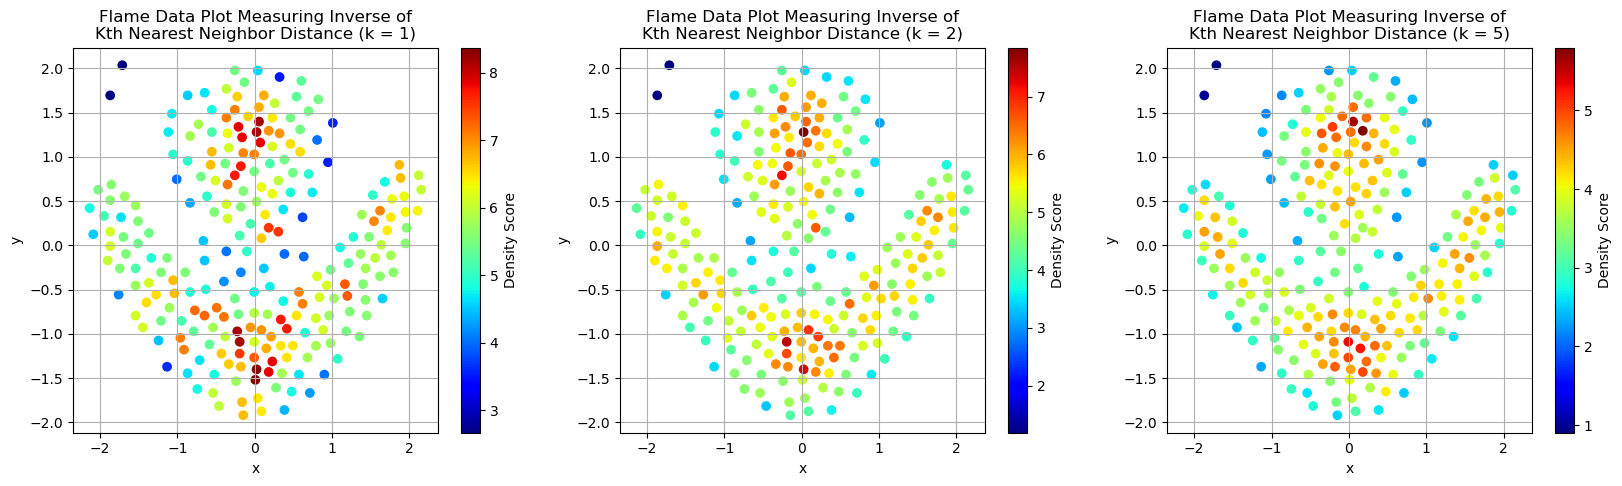
\includegraphics[width=\textwidth]{p3_p2a.png}
    \caption{Flame Data Anomaly Score}
\end{figure}
\begin{figure}[H]
    \centering
    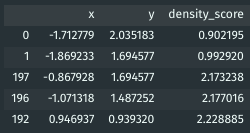
\includegraphics[width=0.4\textwidth]{p3_d2a.png}
    \caption{Flame Data Top 5 Anomalies (k = 5)}
\end{figure}

\begin{figure}[H]
    \centering
    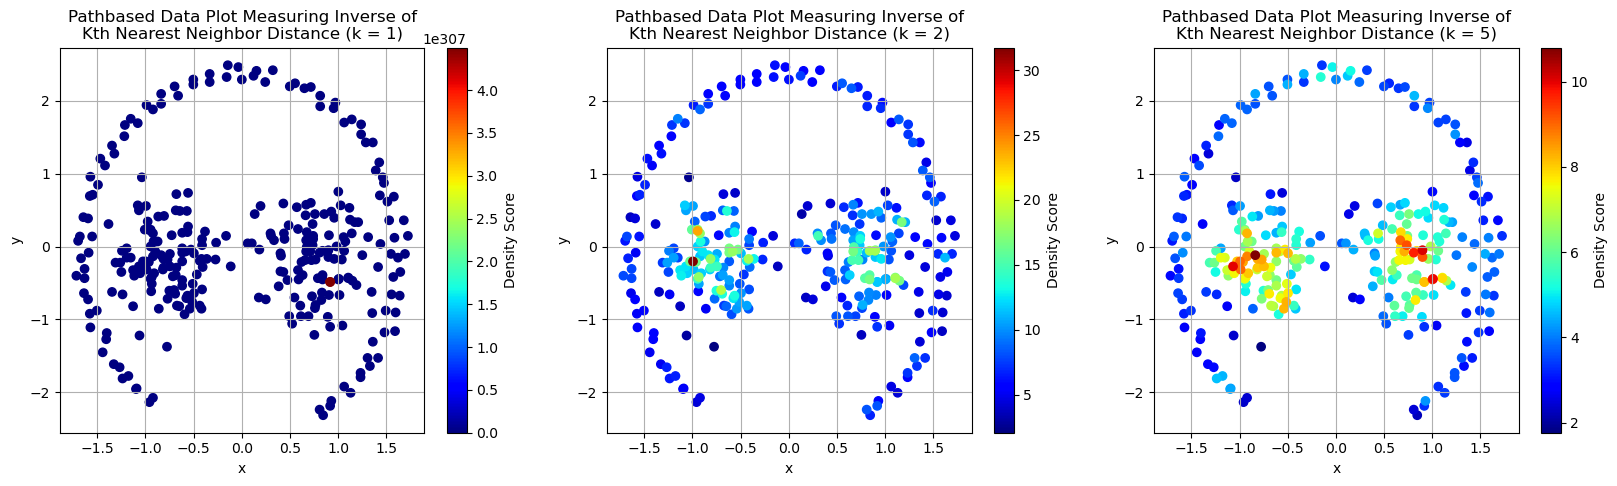
\includegraphics[width=\textwidth]{p3_p3a.png}
    \caption{Pathbased Data Anomaly Score}
\end{figure}
\begin{figure}[H]
    \centering
    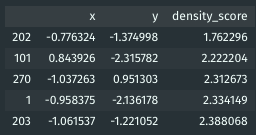
\includegraphics[width=0.4\textwidth]{p3_d3a.png}
    \caption{Pathbased Data Top 5 Anomalies (k = 5)}
\end{figure}

For all above datasets, using the inverse of the distance to the 5th nearest neighbor as
the density measure works best. The points with the shortest distance to the 5th nearest
neighbor end up with a higher density making them less likely to be anomalies. This
results in the anomalies becoming easily identifiable as the coldest points, farthest away
from the warm, densely packed regions.

\subsection{B. Density as the Inverse of the Average of all $k$ Nearest Neighbor Distances}
\begin{figure}[H]
    \centering
    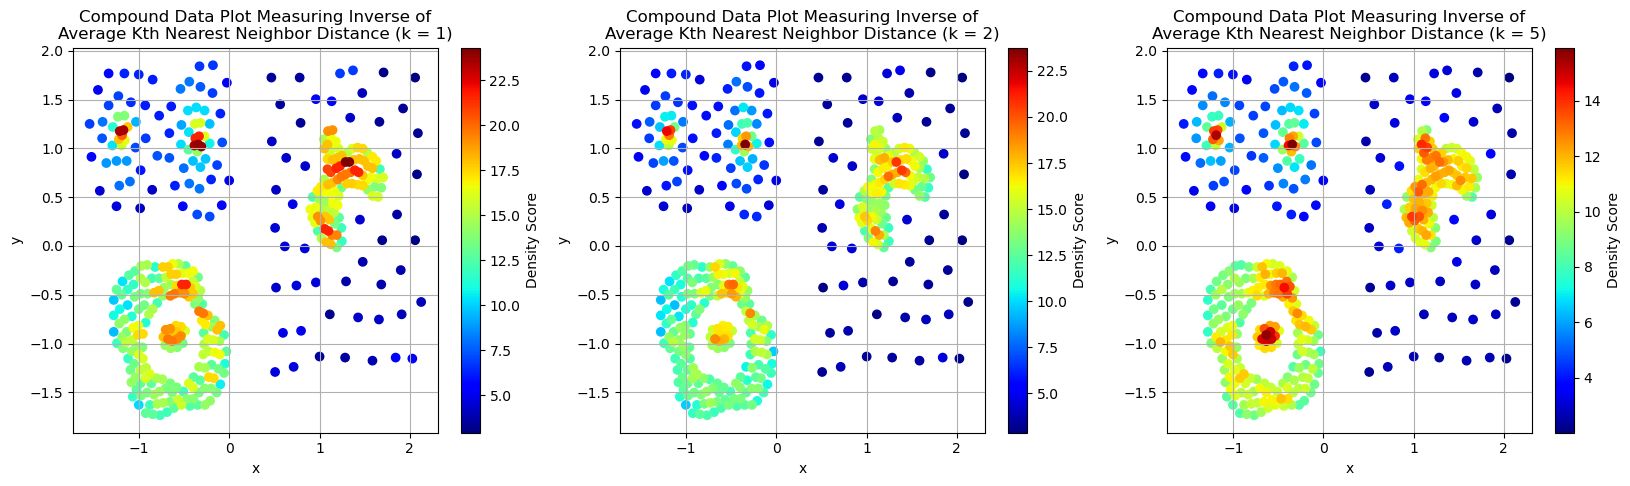
\includegraphics[width=\textwidth]{p3_p1b.png}
    \caption{Compound Data Anomaly Score}
\end{figure}
\begin{figure}[H]
    \centering
    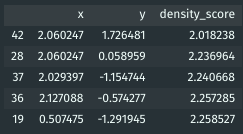
\includegraphics[width=0.4\textwidth]{p3_d1b.png}
    \caption{Compound Data Top 5 Anomalies (k = 5)}
\end{figure}

\begin{figure}[H]
    \centering
    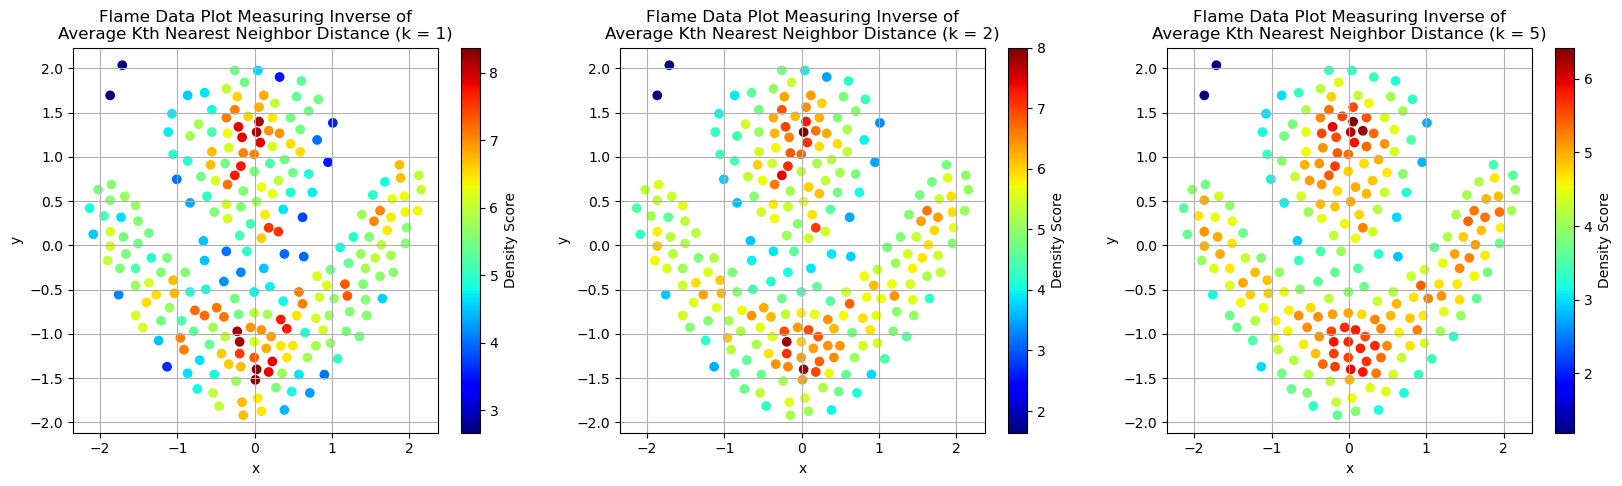
\includegraphics[width=\textwidth]{p3_p2b.png}
    \caption{Flame Data Anomaly Score}
\end{figure}
\begin{figure}[H]
    \centering
    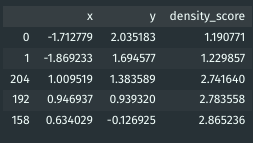
\includegraphics[width=0.4\textwidth]{p3_d2b.png}
    \caption{Flame Data Top 5 Anomalies (k = 5)}
\end{figure}

\begin{figure}[H]
    \centering
    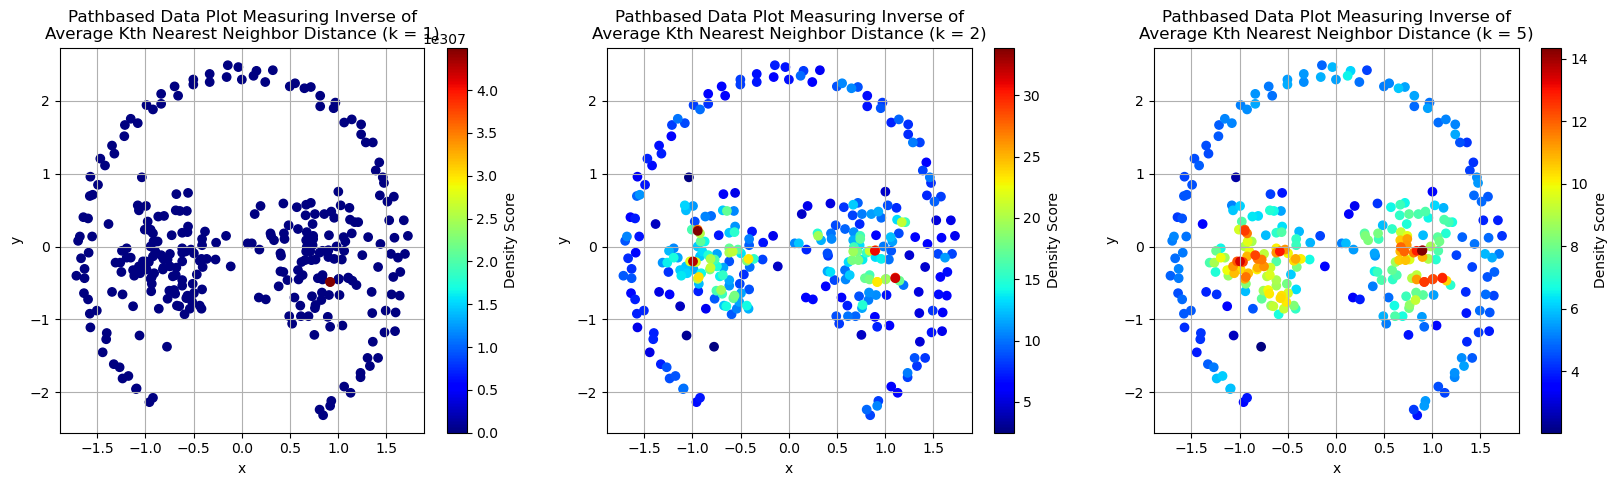
\includegraphics[width=\textwidth]{p3_p3b.png}
    \caption{Pathbased Data Anomaly Score}
\end{figure}
\begin{figure}[H]
    \centering
    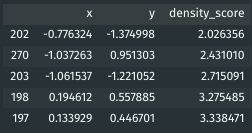
\includegraphics[width=0.4\textwidth]{p3_d3b.png}
    \caption{Pathbased Data Top 5 Anomalies (k = 1)}
\end{figure}

When using the inverse of the average of the distances to all k neighbors, k=5 results in the
best anomaly detection. Here, the densely packed regions and the densest points are easily
differentiable from the low density (high anomaly points). This is especially visible
in the Compound and Flame datasets.

\subsection{Conclusion}
The effectiveness of anomaly detection models depends heavily on the data distribution.
Parametric models like Mahalanobis distance are well-suited for roughly normal distributions,
effectively identifying off-distribution anomalies in datasets like G-Data. For more complex
distributions, distance-based models (e.g., distance to the k$^{th}$ nearest neighbor) and
density-based models (inverse distances) offer robust alternatives. Specifically, using the
distance to the k$^{th}$ nearest neighbor when (k=5) highlights anomalies farthest from
compact clusters, while density-based models, particularly the inverse of the average
distance to k neighbors, excel at distinguishing densely packed regions from sparse
anomalies. Across varied datasets like Compound, Flame, and Pathbased, density-based
scoring with k=5 proved to be the most effective and flexible approach.

\end{document}
